\chapter{\textsc{Analyse du procédé en boucle ouverte}}
\section{\textsc{ Analyse du modèle à temps discret de l'ensemble (bloqueur d'ordre $0$, procédé en boucle ouverte) }}
\subsection{\textsc{La description sur les matrices d'état $ A_d,\hspace{1mm}B_d $ et $ C_d $ }}

De la représentation d'état on trouve :
	\begin{center}
		$ \dot{x}(t)=Ax(t)+Bu(t)$\\
 		$ \Longrightarrow  x(t) = e^{At} x(0) + \overset{t}{\underset{0}{ \int }} e^{ A(t-h)} Bu(h) dh $\\
 		et $y(t)=Cx(t) $
	\end{center}
Soit $T_e$ la période d'échantillonnage, avec: $t \in [kT_e,(k+1)T_e]$, et $u(t)=cste=u$:\\

	\begin{center}
		$ x[(k+1)T_e] = e^{AT_e} x(kT_e) + \overset{T_e}{\underset{0}{ \int }} e^{ A(T_e-h)} Bu(h) dh $\\
 		$ x[(k+1)T_e] = e^{AT_e} x(kT_e) +  \overset{t}{\underset{0}{ \int }} e^{ A(T_e-h)}dh Bu $ \\[0.5 cm]
 		\end{center}
 		
 		Du coup: \\
 		\begin{center}
 		$ x[(k+1)T_e] = e^{AT_e} x(kT_e) + [A^{-1}(e^{AT_e}-I_d)] Bu $ si $A$ est inversible.\\[0.25 cm]
 		et $y(kT_e)=Cx(kT_e)$
	\end{center}
Par identification avec les relations suivantes:\\ 
	\begin{center}
		$ x[(k+1)T_e] = A_d x(kT_e) + B_d u(kT_e) $\\
 		et $y(kT_e)=C_d x(kT_e)$\\
	\end{center}	
On trouve: 
	\begin{center}
		$ A_d = e^{AT_e} $\\
		$ B_d = A^{-1}(e^{AT_e}-I_d) $ si $A$ est inversible.\\  
 		$ C_d = C $
	\end{center}


\chapter{\textsc{Commande du procédé par retour d'état discret}}
\section{\textsc{ Placement des pôles de l'asservissement }}

	\begin{center}
	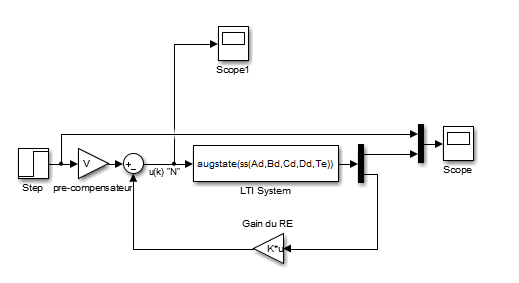
\includegraphics[scale=0.6]{simu1.png}
	\captionof{figure}{\textit{Schéma SIMULINK de l'asservissement avec retour d'état et gain pré-compensateur \\}}
	\label{fig3} 
	\end{center}

\subsection{\textsc{ Asservissment avec F = [$e^{-8T_e} \hspace{1 mm}e^{-8T_e} \hspace{1 mm}e^{-8T_e} \hspace{1 mm}e^{-8T_e}$] }}

Le calcul du gain matriciel du retour d'état $F$ avec la commande MATLAB $acker$ nous donne:
$F = \begin{pmatrix}
	90.9969 \\
	45.5868 \\
	63.3992 \\
	6.5032
\end{pmatrix}$\\

Le calcul du gain pré-compensateur $V$ avec la commande MATLAB $1/dcgain$ nous donne: \hspace{1 cm} $V= 85.5908$. Voir le code MATLAB en annexe.\\
La simulation de la commande $u(k)$ sous SIMULINK avec une consigne qui vaut $e(k)=0.2 m$ nous donne:\\

	\begin{center}
	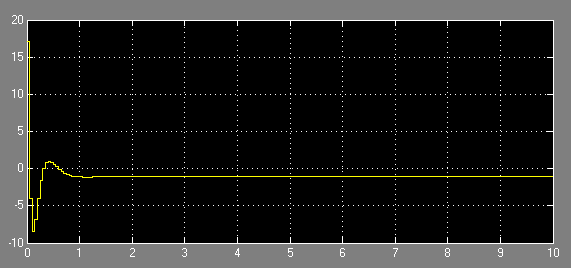
\includegraphics[scale=0.6]{newton1.png}
	\captionof{figure}{\textit{Le SIMULINK de $u(k)$ \\}}
	\label{fig4} 
	\end{center}
	
Cette commande présente un pic qui vaut environ $17.15 N$ ce qui dépasse largement la limite des $6.45N$ imposée auparvant. Cela conclue que cette commande n'est pas acceptable et qu'il faut impérativememnt trouver d'autres pôles.\\

La simulation de la sortie $y_1(t)$ ci-dessous justifie encore plus cette idée car, La variation de l'angle $\alpha$  présente un pic qui vaut $0.251 rad \hspace{1mm} = \hspace{1mm} 14.3^{o}$ et qui représente un angle assez important. L'implémentation sur la maquette vérifie nos prédictions car le rail réagissait violamment à cette commande.       

	\begin{center}
	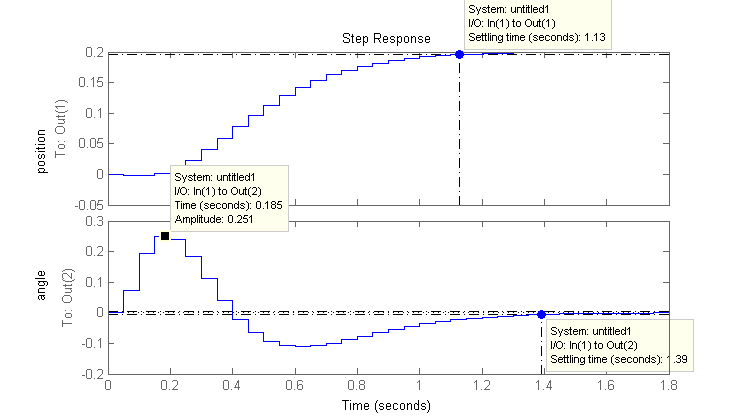
\includegraphics[scale=0.6]{step1.png}
	\captionof{figure}{\textit{La sortie $y_1(k)$ \\}}
	\label{fig5} 
	\end{center} 
	
\subsection{\textsc{ Synthèse de la nouvelle commande }}

Les nouveaux pôles : $ P = [e^{-8Te} \hspace{1 mm}  e^{-10Te} \hspace{1 mm} e^{-2Te} \hspace{1 mm} e^{-4Te}]$ fournissent un gain matriciel $F$ qui vaut:

\begin{center}

$F = \begin{pmatrix}
	   21.6184 \\  16.4050  \\ 36.0568 \\   4.8151
\end{pmatrix}$\\
\end{center}

Et un gain pré-compensateur $V=16.2125$. La suivante simulation de la commande $u(k)$ justifie le choix car elle ne dépasse pas les $6.45N$ imposés. 

	\begin{center}
	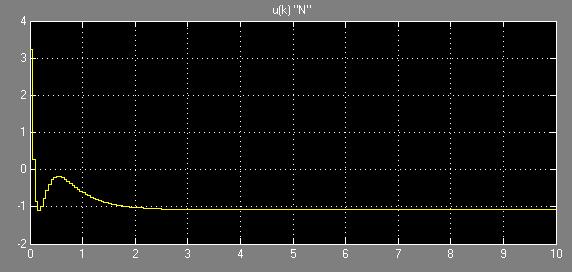
\includegraphics[scale=0.6]{newton2.png}
	\captionof{figure}{\textit{Le SIMULINK de la nouvelle commande $u(k)$ \\}}
	\label{fig6} 
	\end{center}
	
L'implémentation de cette commande devrait réussir avec la nouvelle commande qui possède un bon temps de réponse et un dépassement réduit. 
	
	\begin{center}
	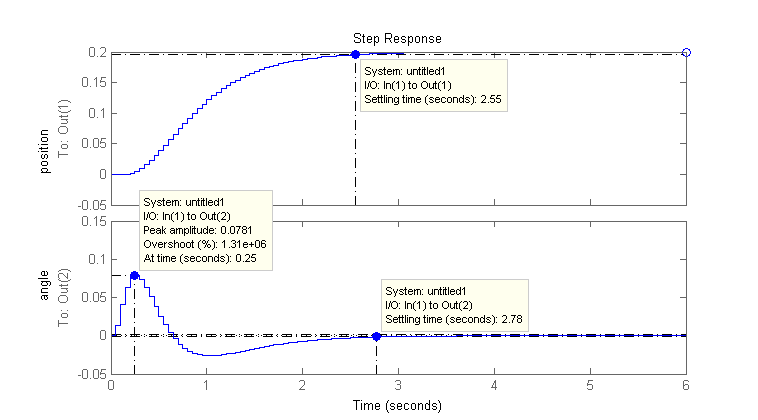
\includegraphics[scale=0.6]{step2.png}
	\captionof{figure}{\textit{La sortie $y_1(k)$ de la nouvelle commande \\}}
	\label{fig7} 
	\end{center}
	
\chapter{\textsc{Estimation des états inaccessibles à la mesure et introduction des états estimés dans la commande}}
\section{\textsc{ Mise en place d'un observateur minimal }}

Les états $x_1(k)$ et $x_3(k)$ état les seuls directement accessibles, on se propose de reconstruire les états $x_2(k)$ et $x_4(k)$ à l'aide d'un observateur minimal identité. Pour cela, on réalise le changement de base:

\begin{center}

$\begin{pmatrix}
	  x_1(k) \\  x_2(k)  \\ x_3(k) \\   x_4(k)
\end{pmatrix}= T \begin{pmatrix}
	  x_1(k) \\  x_3(k)  \\ x_2(k) \\   x_4(k)
\end{pmatrix}$ avec $T=T^{-1}=\begin{pmatrix}
	  1 & 0 & 0 & 0 \\  0 & 0 & 1 & 0  \\ 0 & 1 & 0 & 0\\  0 & 0 & 0 & 1
\end{pmatrix}$
\end{center}

Dans la nouvelle base, la représentation d'état du système discret compris entre $u(k)$ et $ y(k)$ s'écrit alors:


\begin{center}

$\begin{pmatrix}
	  x_1(k+1) \\  x_3(k+1)  \\ x_2(k+1) \\   x_4(k+1)
\end{pmatrix}= A^{'}_d \begin{pmatrix}
	  x_1(k) \\  x_3(k)  \\ x_2(k) \\   x_4(k)
\end{pmatrix} + B^{'}_d u(k)$
\end{center}


 
\begin{center}

$\begin{pmatrix}
	  y_1(k) \\  y_2(k) 
\end{pmatrix}= C^{'}_d \begin{pmatrix}
	  x_1(k) \\  x_3(k)  \\ x_2(k) \\   x_4(k)
\end{pmatrix}$
\end{center}

Avec : $A^{'}_d = T^{-1}A_dT,\hspace{1 mm} B^{'}_d = T^{-1}B_d, \hspace{1 mm} C^{'}_d=C_dT=\begin{pmatrix}
	  1 & 0 & 0 & 0\\ 0 & 1 & 0 & 0 
\end{pmatrix}$. Cette représentation présente l'avantage de retrouver directement dans le vecteur de sortie la partie du vecteur d'état qui est accessible à la mesure.

 \subsection{\textsc{ Les équations de l'observateur minimal identité }}
 
 Les matrices $A_B,F_B,B_B$ et $L_B$ intervenant dans les équations:

\begin{center}
	$z(k+1) =  A_Bz(k) + F_By(k) + B_Bu(k)$\\
	$ (\hat{x}_2(k),\hat{x}_4(k))^T= z(k)+ L_By(k) $
\end{center}
Valent:

\begin{center}
	$  A_B = A_{d22} - GA_{d12} $\\[0.25 cm]  
	$  F_B = A_B G - GA_{d11} + A_{d21} $\\ [0.25 cm]  
	$  B_B = B_{d2} - GB_1 $\\ [0.25 cm]  
	$  L_B = GM $ avec: $M=\begin{pmatrix} 1 & 0 & 0 \\  0 & 1 & 0 \end{pmatrix}$
\end{center}

